\chapter{Optimisation} %Last updated 1-2-2016
\label{ch:optimisation}
In this chapter, different optimisation techniques will be discussed. There are two different kinds of optimisations: local optimisation, where a minimum (or maximum) is found, which may be the minimum within a small area in the function space and which does not have to be the absolute optimum of the function, and global optimisation, where the found minimum (or maximum) is ideally the minimum value of the entire function space \cite{visser2014}. Such a function space can contain multiple local minima but only one of these is the global minimum. A general description of the local and global optimisation techniques is provided in \Cref{sec:diffmethloc,sec:diffmethglo} respectively. The different optimisation techniques are compared in \Cref{sec:techcomp} and two methods are chosen through a trade-off in \Cref{sec:chometh}. Finally, the chosen methods will be described in more detail towards implementation in \Cref{sec:impde,sec:impmbh}. An optimisation problem can either be solved analytically (for simple problems), resulting in a direct solution, or numerically (for more intricate problems), approaching the exact solution \cite{noomen2013}. When comparing different optimisation techniques usually cpu time is traded against the accuracy of the result or the robustness of the method. Often a more accurate or reliable result requires more time and thus increases the cpu time required. From now on only minima are discussed, but every method can also be used to find the maximum.

% Examples of a combination of these techniques and advanced techniques are given in \Cref{sec:advhyb}.  

\section{Local optimisation methods}
\label{sec:diffmethloc}
Local optimisation methods aim to find the local optimum of a function within a limited search space. The methods used are called Nelder-Mead (based on a simplex around the initial guess which then progressing in the direction of the best solution), Newton-Raphson (a gradient technique that requires derivative information and works for 1-dimensional problems, the method moves in the direction of the largest derivative), steepest descent (either along the axes or in an arbitrary direction, similar to Newton-Raphson, but now for 2-dimensions) and \ac{SQP} (an approximation of the function that has to be optimised is provided by a quadratic function, which is evaluated and updated until a local optimum is found or a certain cut-off criterion is met) \cite{noomen2013,musegaas2012}. Local optimisation methods are often fast and accurate, producing good results in a short time. But they only focus on a small area of the function space \cite{boyd2004}. Therefore it is important to define a proper initial parameter value for the local methods (for instance by first using a global optimiser). \\

If many local optimisations are used spread over the entire function search space, the chances that the global optimum is found is increased. A method based on multiple local optimisations is \acf{MBH}. This method uses the fact that local optima tend to be grouped together in many problems. The local optimum of such a group is found by hopping within this group. Once the local optimum of such a group is found, the process starts again, but this time somewhere else in the search space. In this way, the global optimum might be found.

%Convex optimisation can help in this case, even if the problem is non-convex. In convex optimisation, there is a maximum of one global minimum and every local minimum is a global minimum. So if a convex approximation is taken for a non-convex problem and this convex approximation is solved, it will result in an accurate result for the approximation of the non-convex problem. This value can then be used as the initial input for the local optimisation providing a quicker and more accurate result in the end, which could even lead to the global minimum. 


\section{Global optimisation methods}
\label{sec:diffmethglo}
In \cite{noomen2013}, two main numerical global optimisation categories are mentioned: sampling methods and metaheuristics. In global optimisation the minimum value of the complete function is strived for, or at least an approximation of this value.

%Global optimisation is usually used for problems that only have a few variables, because the computation time using these methods can be very long \cite{boyd2004}. 


\subsection{Sampling methods}
\label{subsec:sampmeth}
The sampling methods are based on selecting a value for the variable(s) in the function and then evaluating the function. This is done for many different values until a minimum is found and can be accomplished randomly (Monte Carlo) or using a certain pattern (grid search, Latin hypercube sampling). Because Monte Carlo is based on the evaluation of the function using randomly generated values for the variables, many different points are often required, which increases the required cpu time. Also, the final resolution depends on the resolution of the random number generator. In grid search the value space is divided up into a number of different possible values, where the amount of points depends on the desired resolution. In this case the function is evaluated starting with the first values until each value has been used, and the minimum function evaluation is stored. Again, the number of points is very important and often many are required. Latin hypercube sampling is a method based on matrices \cite{helton2003}, where an n-dimensional matrix is generated such that each random value is only used once in each row and column (for a 2-dimensional case). From this matrix, in case 2-dimensions are used, samples are chosen such that each row and column only provides one sample.\\
The variable values can also be generated quasi-random, which often involves generating all the different values at the start of the optimisation and then evaluating the function for every of these values. An example of such a method is Sobol sequencing \cite{sobol1998}, where all the values are generated using a pre-set function developed by Sobol. Sampling methods can be used to make a rough inventory of the total search space and reduce this for a local optimiser since the resolution of sampling methods can be limited. However, should a sampling method be applied to a small function space, accurate results can still be obtained, which is why it can also be used for local optimisation.

%\subsection{Local optimisation}
%\label{subsec:locopt}
%Local optimisation locates the local minimum (or maximum) of a function. The methods used are called \textbf{Nelder-Mead}, \textbf{Newton-Raphson} (1D), \textbf{steepest descent} (either along the axes or in an arbitrary direction), \textbf{Sequential Quadratic Programming} and \textbf{Monotonic Basin Hopping}. Unfortunately, they might get stuck at the local min- or maximum.

\subsection{Metaheuristics}
\label{subsec:meta}
Metaheuristics are numerical optimisation techniques that directly propagate towards the solution. Unfortunately, full convergence cannot always be achieved, and usually a local optimisation gradient method is required to refine the final solution. The different methods are: \ac{GA}, \ac{DE} (both based on \ac{EA}), \ac{PSO}, (Adaptive) \ac{SA}, Ant Colony optimisation, Dynamic Programming and Interval Analysis \footnote{Usually using a branch and bound method} \cite{noomen2013,musegaas2012}. Often these methods require many iterations to reach a proper solution, however, they can be very robust and do not always require an accurate initial value.

%Most of the times these methods need a lot of iterations to get to a proper solution, but they are very robust and do not need a good initial value.

%(usually using a branch and bound method \cite{wehart1997})

%\subsection{Special techniques}
%\label{subsec:spectech}
%The final special techniques are called Primer vector theory and Q-Law. These techniques are used to optimise thrust and coast arcs for low-thrust trajectories for instance but usually require one of the earlier mentioned optimisation techniques for proper optimisation. 

%\section{Advanced and hybrid techniques}
%\label{sec:advhyb}
%When it comes to advanced techniques and hybrid techniques, experience with different problems is desired. Every problem needs a different combination of techniques to find the most optimal solution and these combinations of techniques depend on the judgement of the person solving the problem. Usually a combination of global and local optimisation methods is used to first find a general solution and then refine this solution to find an exact or close to exact solution. Some of these techniques are: hybrid different metaheuristics, separate evolution/branching, combination of sampling and local optimisation methods, combination of metaheuristics and local optimisation methods, and search space pruning (often used in interval analyses \cite{wehart1997}).



\section{Technique comparison}
\label{sec:techcomp}
To gain a better understanding of the different methods mentioned in  \Cref{sec:diffmethloc,sec:diffmethglo}, a comparison is made between all of them. \Cref{tab:methcomp} shows the advantages and disadvantages of each method using a similar representation as provided in \cite{noomen2013}. For metaheuristics the general advantages are: robust, do not depend on derivatives, do not require a good initial value and propagate directly towards a solution. The general disadvantages are: need many iterations, convergence is unclear and become very slow for a large number of variables. Also, often metaheuristics require a local optimisation method to reach the precise final optimum. In the table the advantages and disadvantages that separate the different metaheuristic methods are mentioned. A global optimum is preferred.

%In the case of launch trajectory and transfer orbit optimisation, a global minimum solution is wanted. Therefore, getting stuck at a local minimum is not advantageous.

%\begin{adjustbox}{width=\textwidth,totalheight=\textheight,keepaspectratio}
%\begin{table}[!ht]
%\begin{center}

\begin{longtable}{|p{2.5cm}|p{1.5cm}|p{6cm}|p{6cm}|}
\caption{Optimisation method comparison \cite{noomen2013} (unless mentioned otherwise).}
\label{tab:methcomp}
\endfirsthead
\endhead
\hline 
\textbf{Method} 		& \textbf{Type} & \textbf{Advantage} & \textbf{Disadvantage} \\ \hline \hline

Nelder-Mead		& Local  & simple & converges to local minimum \\ \hline
Newton-Raphson	& Local & simple & convergence is slow near a flat optimum and converges to local minimum \\ \hline
Steepest descent	& Local  & simple, always finds a minimum and only requires previous gradient information (arbitrary direction results in better conversion) & can oscillate around minimum, has a slow convergence and converges to a local minimum (needs second derivatives/Hessian matrix for arbitrary directions) \\ \hline
\ac{SQP} \cite{boggs1995} 	& Local & works well on non-linearly constrained problems and neither initial point or iterate points have to be feasible & converges to local minimum \\ \hline
\ac{MBH}		& Local/ Global & can locate several local minima that are close together \cite{musegaas2012} & no guarantee that best found local minimum is also global minimum and normal Basin Hopping is preferred when searching one local minimum \cite{iwamatsu2004} \\ \hline 

Monte Carlo 	& Global/ sampling & simple to implement and does not depend on derivatives & only simple problems (otherwise very slow), it is based on luck and can have bad resolution (approximation of value) \\ \hline
Grid search 		& Global/ sampling & simple to implement and does not depend on derivatives & slow and has to trade resolution against cpu time \\ \hline
Latin hypercube sampling \cite{helton2003}		& Global/ sampling & simple to implement, does not depend on derivatives and it provides more regular sampling & only simple problems (otherwise very slow) \\ \hline
Sobol sequencing \cite{sobol1998}		& Global/ sampling & good uniform distribution (regular sampling), faster convergence and does not depend on derivatives  & all sampling values are generated at once, and performs poorly on higher-dimensional problems \\ \hline
\ac{GA}		& Global & simple, easy to understand & original formulation uses binary numbers to encode variables \\ \hline
\ac{DE} 		& Global & simple, uses actual variable values & original \ac{DE} does not perform well for multi-objective problems and was not intended for binary code use \cite{coello2007evolutionary} \\ \hline
\ac{PSO} \cite{selvi2010comparative}		& Global & does not use mutations, very fast, simple, based on intelligence and can be used for multi-objective problems  &  problem has to have a specific structure \\ \hline
\ac{SA} \cite{busetti2003simulated,ingber1993simulated} 		& Global &  easy to program, can be applied to many different problems, can deal with many constraints &  fine-tuning of the constraints and variables can be delicate, often requires much storage space and cpu time \\ \hline
Ant Colony Optimisation \cite{selvi2010comparative}	& Global & can be solved using parallel computations, can handle dynamic problems  & based on a sequence of dependent random decisions, and works best for experimental problems  \\ \hline
Dynamic Programming \cite{bhowmik2010}		& Global & solving sub-problems to find problem solution and stores solutions to sub-problems as to only evaluate every sub-problem once & can require much storage space with increase of different sub-problems \\ \hline 
Interval Analysis \cite{horst1995handbook}	& Global & includes different error estimations, can be used for infinite data sets & can be complex \\ \hline 
% 		&  &  &  \\ \hline
\end{longtable}
%\end{center}
%\end{table}
%\end{adjustbox}


%Primer vector theory 		& Global & specific applications for space problems, precise and can be used for many general cases \cite{musegaas2012} & can become sensitive if more gravity assists are added \\ \hline 
%Q-law 		& Global & specific applications for space problems & needs metaheuristics for Optimisation \cite{lee2005} \\ \hline 
%Separate evolution /branching 		& Global & spreads optimisation over several processors and more computations done  \cite{musegaas2012}& refinement of solution might be needed and requires several processors  \\ \hline
%Search space pruning 		& Local and Global & more focussed search (quicker) & requires good knowledge of the problem and can become very complex if number of levels increase \cite{musegaas2012} \\ \hline

%Also, the metaheuristic (and other global) methods usually require extra optimisation by using a gradient technique to get (close to) the exact minimum value.  


\section{Chosen methods}
\label{sec:chometh}
It is important to use an optimisation method that is best suited for the thesis problem, or a method that shows potential in becoming the best optimisation method for this particular kind of problem. The thesis problem might use two different methods and compare the performance of these methods or even combine them to produce an even more suited method. It could also be that simply one optimisation method is chosen and the focus of the thesis will be put on other aspects. This final decision of what to focus on will be made in \Cref{ch:findef}. To accommodate this decision, two optimisation methods (out of the ones provided in \Cref{tab:methcomp}) will have to be selected. To reduce the amount of method used in the trade-off and to help establish the different criteria, reference research and TU Delft (Space department) heritage will be used. Basing the decision on what knowledge already exists in the department would allow for use of resources that are already available and would make it easier to learn from experienced people. However, other used methods for similar subject problems could not be ignored, since one method might be better suited for the problem than the other. Therefore, \Cref{subsec:freqmeth} first describes a collection of methods that have frequently been used for similar problems and then \Cref{subsec:tuher} will discuss several methods used in the Space department. The final trade-off will be described in \Cref{subsec:chocanmeth}.

\subsection{Frequently used methods}
\label{subsec:freqmeth}
The required method depends on the problem that needs to be solved. To help determine which methods to use for the thesis problem, reference optimisation research was consulted. An overview is presented in \Cref{tab:prevmeth}. In this case only research focused on finding the global optimum is provided because the thesis problem will also focus on finding the global optimum. Most of the problems mentioned in \Cref{tab:prevmeth} required metaheuristic methods. Addis et al. \cite{addis2011} mentions that \ac{DE} is very popular because of its robustness resulting in good results, but that \ac{MBH} might be a better alternative because it can produce even better results. 


%to be able to quickly see who used what method for what particular purpose, it is best to have an overview as was done in \Cref{sec:techcomp}. Therefore \Cref{tab:prevmeth} has been set-up to show a selection of similar research and the methods used. They are mentioned in chronological order of publication; earliest publication first. 

\begin{table}[!ht]
\begin{center}
\caption{Previous methods used for trajectory and orbit transfer optimisation problems.}
\label{tab:prevmeth}
\begin{tabular}{|p{5cm}|l|p{5cm}|p{5cm}|}
\hline 
\textbf{Author} 		& \textbf{Year} & \textbf{Subject} & \textbf{Method} \\ \hline \hline
Gage et al. \cite{gage1995} & 1995		& Interplanetary Trajectory (Mars missions) & \ac{GA}  \\ \hline
Rauwolf and Coverstone-Carroll \cite{rauwolf1996} 		& 1996 & Low-thrust orbit transfers (to Mars and Mercury) & \ac{GA}  \\ \hline
Kim and Spencer \cite{kim2002} & 2002		& Spacecraft Rendezvous  & \ac{GA}s  \\ \hline
Myatt et al. \cite{myatt2004} 	& 2004	& Mission Analysis and Design (transfer orbits) & \ac{DE} (most robust)  \\ \hline
Lee et al. \cite{lee2005} & 2005		& Low-thrust orbit transfers &  Q-law with \ac{GA} and Q-law with \ac{SA} \\ \hline
Abdelkhalik and Mortari \cite{abdelkhalik2007} & 2007 & Transfer orbits &  \ac{GA}s \\ \hline
Vasile et al. \cite{vasile2008} & 2008		& Space trajectories & \ac{MBH}  \\ \hline
Garcia et al. \cite{garcia2010} & 2010		& Optimisation of Mars entry vehicle for a mass of 40 tons & (Multi Objective) \ac{GA}  \\ \hline
Li and Peng \cite{shuang2011} 	& 2011	& Mars entry and descent &  \ac{SQP} and Monte Carlo \\ \hline
Addis et al. \cite{addis2011} & 2011		& Space trajectories &  \ac{MBH} \\ \hline

 		
% 		&  &   \\ \hline
\end{tabular}
\end{center}
\end{table}



%When looking at the problem of ascent launch trajectory optimisation again metaheuristics can be used, because they are easy to implement. However, there are some (\cite{betts1998}) who say that when looking at an ascent problem, trajectory optimisation will give the best results when performed analytically (as also done in \cite{visser2014}). This because ascent trajectory optimisation problems do not have discrete variables according to \cite{betts1998}. 


\subsection{TU Delft optimisation heritage}
\label{subsec:tuher}
At the Space department of the TU Delft, a toolbox was developed called Tudat. This toolbox can be used to solve a variety of (aspects of) astrodynamic problems. Within this toolbox, an optimisation toolbox is used called \ac{PaGMO}, which houses a selection a selection of optimisers mentioned in \Cref{tab:methcomp} and more \cite{boudestijn2014}. Since the introduction of this toolbox, students have been working on these optimisation programs within this toolbox, often adjusting it slightly to fit their specific needs. A program using a \ac{PaGMO} optimiser was developed by Musegaas \cite{musegaas2012}. These developed programs were also adjusted to incorporate specific problem needs such as was done by Miranda \cite{miranda2015} where the original program used \ac{DE} and \ac{PSO} was added to produce a better solution. It is however unlikely that Tudat programs itself will be used during this thesis, nonetheless the experience is there and can still be used. An overview of the different research performed by previous master students and the used (and best) optimisation methods is provided in \Cref{tab:prevmethtu}.


\begin{table}[!ht]
\begin{center}
\caption{Previous master theses on trajectory and orbit transfer optimisation problems.}
\label{tab:prevmethtu}
\begin{tabular}{|l|l|p{5cm}|l|}
\hline 
\textbf{Author} 		& \textbf{Year} & \textbf{Subject} & \textbf{Method} \\ \hline \hline
Pagano \cite{pagano2010global} & 2010 & Launch trajectories& \ac{PSO} \\ \hline
Musegaas \cite{musegaas2012} & 2012 & Space Trajectories (including gravity assists and manoeuvres) & \ac{GA}, \ac{PSO} and \ac{DE} (best) \\ \hline
Vandamme \cite{vandamme2012assisted}  & 2012 & Launch trajectories & \ac{PSO} and \ac{DE} (best)   \\ \hline
van Kesteren \cite{kesteren2013air} & 2013 & Launch trajectories & \ac{GA}, \ac{PSO} and \ac{DE} (best) \\ \hline
Boudestijn \cite{boudestijn2014} & 2014 & Low-thrust trajectories & \ac{DE} \\ \hline
Gomez \cite{gomez2015optimization} & 2015 & Low-thrust trajectories & \ac{DE} \\ \hline
Miranda \cite{miranda2015} & 2015 & Hybrid rockets & \ac{DE} and \ac{PSO} (best) \\ \hline
 		
% 		&  &   \\ \hline
\end{tabular}
\end{center}
\end{table}


\subsection{Chosen candidate methods}
\label{subsec:chocanmeth}
The decision of which methods to use will be based on the heritage, reference research, problem type (here launch and space trajectories), accuracy, speed, robustness, easy implementation and novelty. Also, the more resent the research the more relevant it is deemed to be. Based on \Cref{tab:prevmeth,tab:prevmethtu} it was decided to include \ac{GA}, \ac{PSO}, \ac{DE} and \ac{MBH} in the trade-off. The trade-off is visualised using \Cref{tab:opt_trade_off}. Every criterion is assigned a weight depending on how important the criterion is. Then the different methods are either green (1), yellow (0.5) or red (0) for every criterion. This results in a final score. 



\begin{table}[!ht]
\begin{center}
\caption{Optimiser trade-off table.}
\label{tab:opt_trade_off}
\begin{tabular}{|l||l|l|l|l|l|l|l|l||l|}
\hline 
 &	\textbf{Heritage} & \textbf{Ref. research} & \textbf{Trajectories} & \textbf{Accuracy} & \textbf{Speed} & \textbf{Robust} & \textbf{Impl.} & \textbf{Novelty} & \textbf{Score}\\ \hline 
\textit{Weight} & \textit{4} & \textit{4} & \textit{5} & \textit{4} & \textit{3} & \textit{3} & \textit{2} & \textit{5} & \\ \hline \hline
\textbf{\ac{GA}} & \cellcolor{red} & \cellcolor{green} & \cellcolor{yellow} & \cellcolor{yellow} & \cellcolor{yellow} & \cellcolor{yellow} & \cellcolor{green} & \cellcolor{red} & 13.5 \\ \hline
\textbf{\ac{PSO}} & \cellcolor{yellow} & \cellcolor{red} & \cellcolor{yellow} & \cellcolor{yellow} & \cellcolor{green} & \cellcolor{yellow} & \cellcolor{green} & \cellcolor{yellow} &  15.5 \\ \hline
\textbf{\ac{DE}} & \cellcolor{green} & \cellcolor{green} & \cellcolor{green} & \cellcolor{yellow} & \cellcolor{yellow} & \cellcolor{green} & \cellcolor{green} & \cellcolor{yellow} & 24  \\ \hline
\textbf{\ac{MBH}} & \cellcolor{red} & \cellcolor{green} & \cellcolor{green} & \cellcolor{green} & \cellcolor{yellow} & \cellcolor{green} & \cellcolor{green} & \cellcolor{green} & 24.5 \\ \hline

\end{tabular}
\end{center}
\end{table}


Currently, the method that is used most is \ac{DE}, which also results in a high score in the trade-off table. However based on the reference research it is clear that even though \ac{DE} is very popular even outside of the TU Delft, \ac{MBH} could be an attractive alternative. Indeed, \ac{MBH} scored similarly to \ac{DE} in the trade-off (and even slightly better). This is why it was decided to investigate both \ac{DE} and \ac{MBH}. This is also interesting from an academic point of view, since there is currently a discussion on which method is better for trajectory problems. The next two sections will discuss each of the chosen methods in more detail and explain how they can be implemented.

\section{Implementation of \ac{DE}}
\label{sec:impde}
\acl{DE} is a direct global method based on \ac{EA}s and was first introduced by Storn and Price back in 1995 \cite{storn1995differential}. The method became increasingly popular after performing well in two world-wide optimisation competitions \cite{price2005differential} and finally caught the interest of the scientific and engineering community in 1997 when two more papers were published of which the final paper \cite{storn1997differential} provided a clear and easy-to-understand description of the method. This description will also be used in \Cref{subsec:workde} to explain the basics of \ac{DE}. In \Cref{subsec:vardemeth} variations on the original \ac{DE} method are explained.


\subsection{Workings of \ac{DE}}
\label{subsec:workde}
When using \ac{DE} for a minimisation problem the objective is to find the minimum global function evaluation. For instance, if the aim is to find the minimum propellant mass to reach a certain point in a certain orbit then the function will be written to compute the required propellant mass given a combination of different variables (such as launch azimuth and lift-off mass). These variables values are initially randomly chosen by the \ac{DE} algorithm and their combination is optimised to reach a minimum propellant mass solution. In such a case, the minimum propellant mass function is called the cost function. Because \ac{DE} is based on \ac{EA}s it works with "individuals", "population size", and "generations". An individual is a vector, with all the different variables in it, of size $D$ (the number of variables). The values of these variables are initially randomly chosen for each individual before the \ac{DE} optimisation, within the different variable constraints (parameter space). The population size ($NP$) determines the number of individuals used during the optimisation. Before the start of the optimisation the first generation is generated randomly within the mentioned constraints. Each time an optimisation run is performed, a new generation ($G$) is created with new (improved) individuals, or including the best individuals of the previous generation depending on how well they performed. This means that the optimisation will run until a maximum number of generations is achieved, which means that the maximum number of generations is a set value by the user. The individual vectors per generation can be written as shown in \Cref{eq:individual vector} \cite{storn1997differential}.

\nomenclature[R1]{$D$}{Number of variables\nomunit{-}}
\nomenclature[R8]{$NP$}{Population size\nomunit{-}}
\nomenclature[R4]{$G$}{Generation\nomunit{-}}


\begin{equation} \label{eq:individual vector}
x_{i,G} \quad \text{with} \quad i = 1,2,\dotsc,NP
\end{equation} 

\nomenclature[Ra6]{$x_{i,G}$}{Original, target, individual vector\nomunit{-}}

To generate new individual vectors during the optimisation (new generation), \ac{DE} adds the weighted difference between two individual vectors to a third vector, a process called mutation, and then mixes this new mutation vector $v_{i,G+1}$ with the original, target, individual vector $x_{i,G}$ resulting in a trial vector $u_{i,G+1}$, a process called crossover. Here, the three individual vectors used to compile the mutation vector are all distinctly different from the original individual vector. This then calls for the requirement that $NP$ is at least equal to 4. 
In equation form this means that first the mutant vector is created through the use of \Cref{eq:mutation vector} (visualized for a two-dimensional cost function in \Cref{fig:mut_vec_storn1997differential}). 

\nomenclature[Ra2]{$v_{i,G+1}$}{Mutation vector\nomunit{-}}
\nomenclature[Ra2]{$u_{i,G+1}$}{Trial vector\nomunit{-}}

\begin{equation} \label{eq:mutation vector}
v_{i,G+1}=x_{r_{1},G}+F\cdot\left(x_{r_{2},G}-x_{r_{3},G}\right)
\end{equation}

\nomenclature[R3]{$F$}{Amplification factor\nomunit{-}}


\noindent where in \Cref{eq:mutation vector} $r_{1}, r_{2},r_{3}\in \left\lbrace 1,2,\dotsc,NP \right\rbrace$ are all different and different from $i$. Also $F\in \left[0,2 \right]$, where $F$ is called the amplification factor (or weight) which determines the impact of the difference vector to the first chosen $x_{r_{1},G}$ vector and is selected by the user. It should be noted that in case of a strictly constraint problem, such as the proposed thesis topic problem (constraints on \ac{MAV} design), each of the new variables created through mutation should be checked for plausibility. This means that the value for the different variables should always be within the respective parameter space.  

\begin{figure}[!ht]
\centering
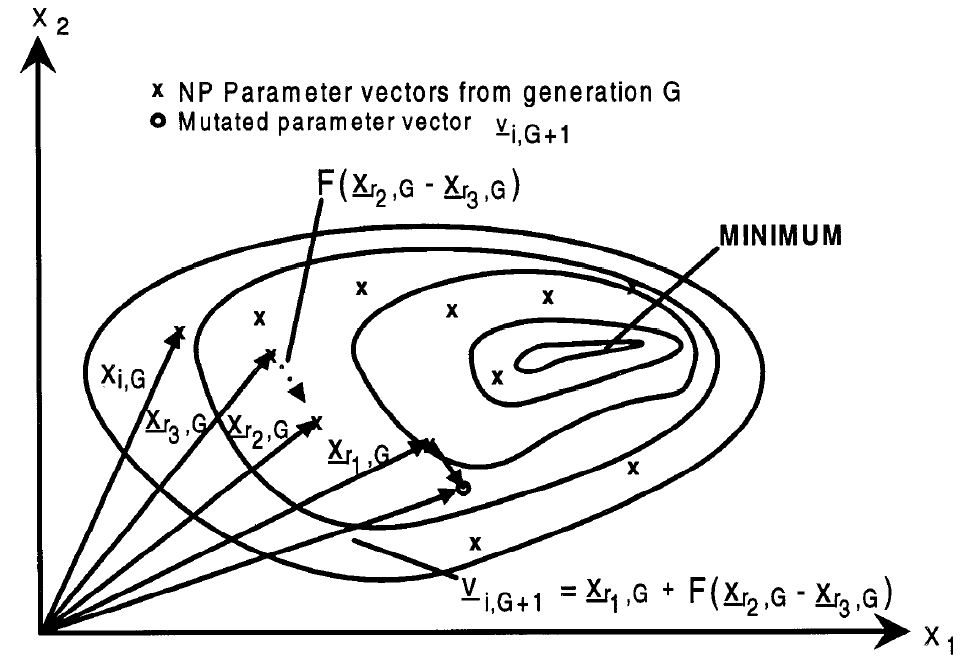
\includegraphics[width=0.5\textwidth]{figures/optimisation/mut_vec_storn1997differential.jpg}
\caption{Construction of the mutation vector in a two-dimensional case \cite{storn1997differential}.}
\label{fig:mut_vec_storn1997differential}
\end{figure}

The crossover/trial vector is composed of the variables from both $x_{i,G}$ and $v_{i,G+1}$. Each different variable is denoted by its separate position number $j$ (thus $j=1,2,\dotsc,D$). Using this notation the trial vector can be described as $u_{i,G+1}=\left(u_{1i,G+1},u_{2i,G+1},\dotsc,u_{Di,G+1} \right)$ where the determination of which variable value originates from which vector ($x_{i,G}$ or $v_{i,G+1}$) is determined by \Cref{eq:trial vector} and visualized by \Cref{fig:trial_vec_storn1997differential} for a 7-dimensional case.

\begin{equation} \label{eq:trial vector}
u_{ji,G+1}=\begin{cases}
v_{ji,G+1}, & \textbf{if}\ \left(randb\left(j\right)\leq CR \right) \ \textbf{or}\ j=rnbr\left(i\right)\\
x_{ji,G}, & \textbf{if}\ \left(randb\left(j\right)>CR \right) \ \textbf{and}\ j\neq rnbr\left(i\right)
\end{cases}\\
\end{equation}

\nomenclature[R1]{$CR$}{Crossover constant\nomunit{-}}


\begin{figure}[!ht]
\centering
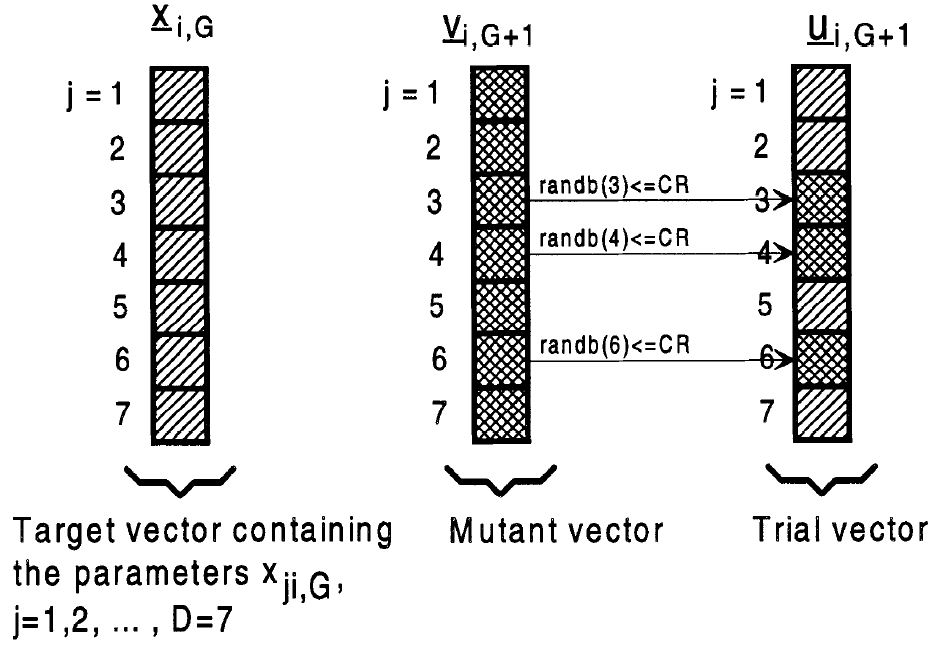
\includegraphics[width=0.3\textwidth]{figures/optimisation/trial_vec_storn1997differential.jpg}
\caption{Construction of the trial vector in a 7-dimensional case \cite{storn1997differential}.}
\label{fig:trial_vec_storn1997differential}
\end{figure}

\noindent where in \Cref{eq:trial vector} $randb\left(j\right)\in \left[0,1\right]$ and is the j$^{th}$ evaluation obtained from a  uniform random generator \cite{storn1997differential}. Also, $CR$ is called the crossover constant which is chosen by the user $\in \left[0,1\right]$ and $rnbr\left(i\right)$ is again a random chosen number. This ensures that at least one variable from the mutation vector will become part of the trial vector. The last step is to determine whether the trail vector $u_{i,G+1}$ generates a better value, or lower propellant mass in case of the example, than the original, target, individual vector $x_{i,G}$. If the trial vector performs better, then the i$^{th}$ individual vector in the next generation $x_{i,G+1}$ becomes $u_{i,G+1}$. However, if it performs worse than $x_{i,G}$, then $x_{i,G+1}$ becomes $x_{i,G}$. This is done for every individual vector in the population. Once the entire population in a generation has been examined, and has either been replaced by a better combination or not, the next generation is examined until the final generation is reached.
A pseudo-code for this process written in C is provided in the paper of Storn and Price \cite{storn1997differential} and a specific example of this \ac{DE} application is presented in \cite{feoktistov2006differential} for both C and Matlab.  

%\nomenclature{}{Description\nomunit{$-$}}

\subsection{Variations of \ac{DE}}
\label{subsec:vardemeth}
In their 1997 publication, Storn and Price also mention that the \ac{DE} method described in \Cref{subsec:workde} is not the only way to implement \ac{DE}. In fact they make a selection of three distinct changes that can be made to vary the method. The first change would be that, instead of taking a random individual vector $x_{r_{1},G}$ as the vector that will be mutated shown in \Cref{eq:mutation vector}, one could also mutate the best individual vector (so the individual vector with the lowest value for the cost function that is not equal to the current ($i$) vector being examined). In that case \Cref{eq:mutation vector} would change to \Cref{eq:best_mutation vector}.

\begin{equation} \label{eq:best_mutation vector}
v_{i,G+1}=x_{best,G}+F\cdot\left(x_{r_{1},G}-x_{r_{2},G}\right)
\end{equation}

The second change would be to use more difference vectors. In the case of \Cref{eq:mutation vector,eq:best_mutation vector} only one difference vector is used. Should, for instance, two difference vectors be used then \Cref{eq:best_mutation vector} would change into \Cref{eq:best_2mutation vector} \cite{storn1997differential}.
This would however also affect the constraint for NP, which would in this case increase to a minimum of 6 (every added difference vector raises the minimum NP by 2).


\begin{equation} \label{eq:best_2mutation vector}
v_{i,G+1}=x_{best,G}+F\cdot\left(x_{r_{1},G}+x_{r_{2},G}-x_{r_{3},G}-x_{r_{4},G}\right)
\end{equation}

The final change would be in how the crossover is determined. Currently this is done using an independent binary (bin) experiment. The notation used to differentiate between the different options would be DE/rand/1/bin for the method described in \Cref{subsec:workde}, DE/best/1/bin if \Cref{eq:best_mutation vector} were to be used and if \Cref{eq:best_2mutation vector} would be used, the notation would change to DE/best/2/bin, just to give a few examples.\\

Concerning the different control variables ($NP$, $F$ and $CR$), a different optimiser could also be incorporated to optimise these parameters each time to gain the fastest result depending on the kind of problem. Storn and Price \cite{storn1997differential} do, however, provide a fair range and approximation of values for the control variables. As by Storn and Price: "$F$ =
0.5 is usually a good initial choice. If the population converges prematurely, then $F$
and/or $NP$ should be increased. Values of $F$ smaller than 0.4, like those greater than
1, are only occasionally effective. A good first choice for $CR$ is 0.1, but since a
large $CR$ often speeds convergence, to first try $CR$ = 0.9 or $CR$ = 1.0 is appropriate
to see if a quick solution is possible. For fastest convergence, it is best
to pick the initial parameter range such that it covers the region of the suspected global optimum,
although this choice doesn’t seem to be mandatory." They also mention that a reasonable choice for $NP$ is between 5 times $D$ and 10 times $D$, however $NP$ should always suffice to the minimum requirement as per number of difference vectors. \\

A more recent publication by A. Qing in 2009 \cite{qing2009differential} shows a clear overview of the advances in the field of \ac{DE} since 1997. In this book four different \ac{DE} categories are described: classic, dynamic, modified and hybrid. Classic is the classic method described in \Cref{subsec:workde} and slight modifications to it. As already mentioned it is important to deal with the fact that variables might need to stay within a certain parameter space. Qing describes two methods to deal with mutants that are not feasible: random reinitialization (where a new random variable is generated if the current variable is invalid) and bounce-back (where the value of the variable is brought back into the parameter space on either the lower bound or the upper bound, depending on where it left the parameter space). It is also mentioned that should the optimum be known, the program can be terminated whenever the solution is found within a certain accuracy. The program could also be terminated if the population diversity is very small (smaller than a set limit).This means that almost all the individuals are the same and a solution might not be found. In \cite{qing2009differential} it is mentioned that Storn and Price recommend that $NP$ = 10 times $D$, $F$ = 0.8 and $CR$ = 0.9. However, $F$ = 0.5 and $CR$ = 0.1 are also claimed to be a good first choice, which is similar to the recommendations found in \cite{storn1997differential}. \cite{qing2009differential} also states that it is claimed that convergence is more likely to occur but generally takes longer with larger populations and weaker mutation (smaller $F$). $CR$ = 1 results in faster convergence if convergence occurs but $CR$ = 0 is required to make DE robust enough for particular problems. Dynamic \ac{DE} is similar to classic but is not based on generations. Dynamic \ac{DE} has one population where the better children continuously replace the parents until a certain number of function evaluations has been reached. Also, the best individual is immediately updated every iteration round. Because it is all part of the new iteration, computations cannot be done in parallel any more. In modified \ac{DE} one or several of the following core aspects of classic \ac{DE} is modified: population initialization, differential mutation, crossover, objective and constraint function evaluation, and selection. An example of modified \ac{DE} is provided in \cite{feoktistov2006differential}. And finally hybrid \ac{DE} involves combining \ac{DE} with a deterministic and/or a stochastic optimiser \cite{qing2009differential}. Qing also shows different ways to determine the control parameters $NP$, $F$ and $CR$, plus different ways to perform a multi-objective \ac{DE}, where one would like to optimise different objectives at the same time.\\

It is clear that \ac{DE} is flexible and can be adjusted to different kinds of problems, and what specifically to change depends on the user and the problem itself. It is the choice of the user to specify in what kind of configuration \ac{DE} is to be used. 



\section{Implementation of \ac{MBH}}
\label{sec:impmbh}
\acl{MBH} is an optimisation method initially developed by Leary in 2000 \cite{leary2000global} based on Basin Hopping first introduced by Wales and Doye in 1997 \cite{wales1997global}. It depends on many local optimisations to eventually find a global optimum \cite{vasile2008,musegaas2012,englander2014tuning}, which is why it can also be classified as a combination of a local and global optimiser (depending on the chosen definition). In 2008 Addis et al. \cite{addis2008global} states that \ac{MBH} outperforms \ac{DE} for given optimisation problems, which makes comparing these two methods for this particular thesis topic very interesting. In \Cref{subsec:workmbh} the workings of \ac{MBH} will be explained and any available variations on this method will be discussed in \Cref{subsec:varmbhmeth}.



%Based on Basin-Hopping first introduced by Wales and Doye in 1997 \cite{wales1997global} according to \cite{musegaas2012}. In 2000 an adaptation to this method was introduced by Leary in 2000 \cite{leary2000global} according to \cite{englander2014tuning,musegaas2012,addis2008global,addis2011}.

\subsection{Workings of \ac{MBH}}
\label{subsec:workmbh}
The basic form of \ac{MBH} is probably best explained through the description provided in \cite{englander2014tuning}. The method begins by setting a so-called improvement counter to zero: $N_{n,i}=0$. This counter is used to determine how many times a local optimisation does not result in a better solution than the existing best minimum. Then a set of randomly chosen variable values is generated to use as an initial point/guess. This initial guess vector is called $x$ and is used as the first input for a (by the user) chosen local optimiser. This local optimiser then tries to determine the local minimum point $x^{*}$ (also called a "basin"), and if it finds a feasible solution, this local minimum is set as the current point and called $x_{current}$. If the local optimiser does not find a feasible solution, the program starts over again and chooses a new random point to serve as a new initial guess. This first step is visualized in \Cref{fig:mbh_explained_1} for a one-dimensional case.

%, from within the function space,

\nomenclature[R8]{$N_{n,i}$}{Number of not improved iterations \nomunit{-}}

\begin{figure}[!ht]
\centering
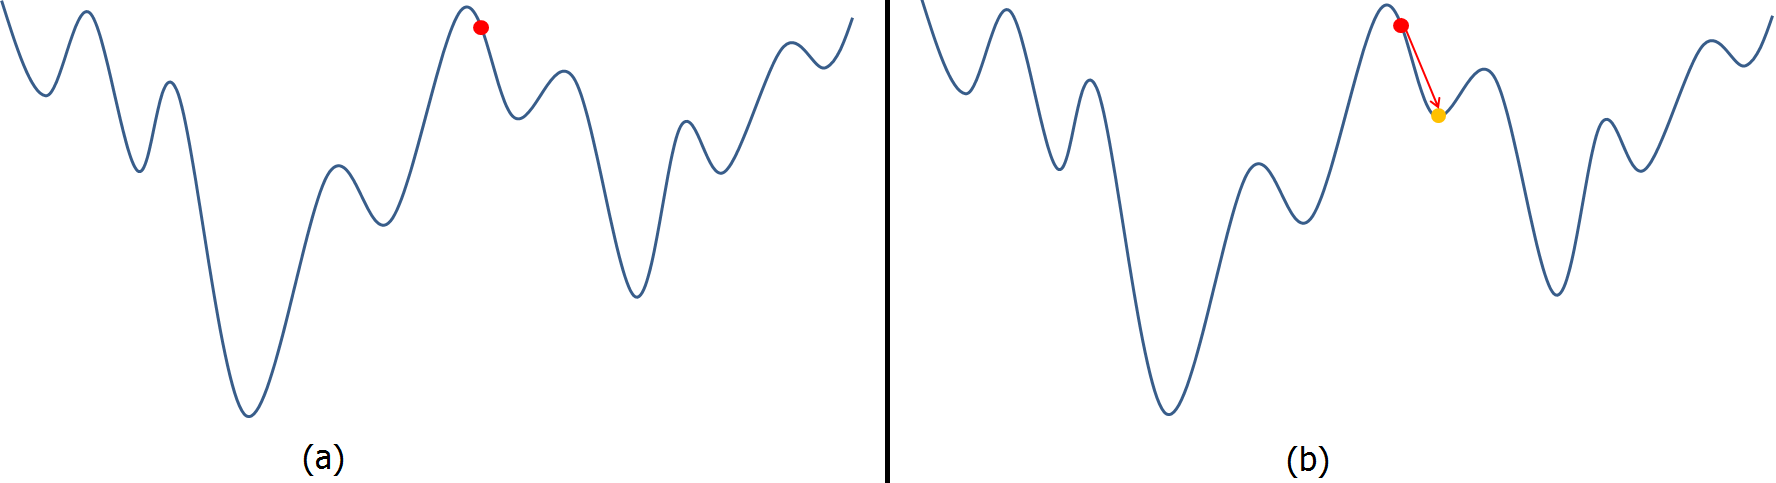
\includegraphics[width=1.0\textwidth]{figures/optimisation/mbh_explained_1.png}
\caption{The first step of \ac{MBH} where (a) first a random initial point $x$ (red dot) is generated after which (b) the local minimum $x^{*}$ (dark yellow point) is found through the use of a local optimiser. The local optimisation is visualized by a solid arrow. $x^{*}$ becomes $x_{current}$ if the local optimum is feasible.}
\label{fig:mbh_explained_1}
\end{figure}

The second step is to perturb (or mutate as it is called in Evolutionary algorithms) $x_{current}$ such that a new vector with variable values, called $x'$, is created. This perturbation is achieved by randomly choosing a deviation of the variable value through the use of a uniform probability distribution in $\left[-\sigma, \sigma \right]$, where $\sigma$ is the standard deviation. This process is visualized in \Cref{fig:mbh_explained_2}.

\nomenclature[G6]{$\sigma$}{Standard deviation \nomunit{-}}

\begin{figure}[!ht]
\centering
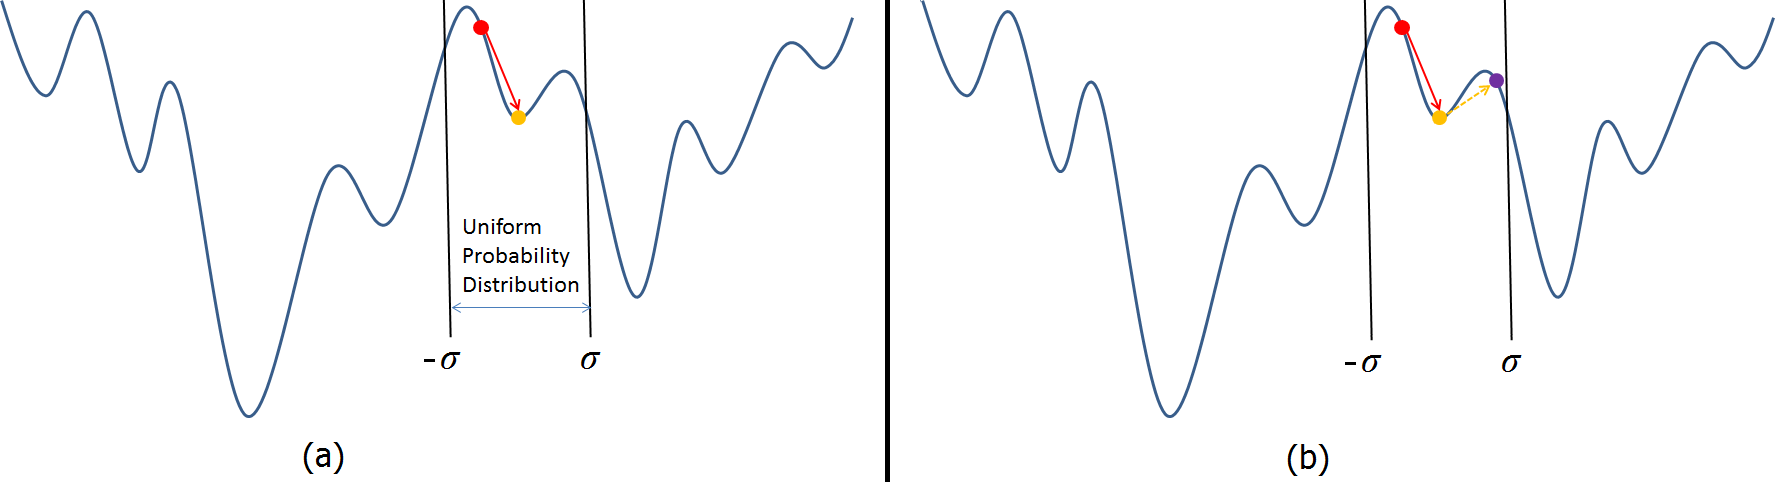
\includegraphics[width=1.0\textwidth]{figures/optimisation/mbh_explained_2.png}
\caption{The second step of \ac{MBH} where (a) $x_{current}$ is perturbed within a uniform probability distribution creating (b) a new initial point $x'$ (purple dot). The perturbation is visualized by a dashed arrow.}
\label{fig:mbh_explained_2}
\end{figure}

Using this new initial point, the local optimiser is run again. If this new $x^{*}$ is feasible \textit{and} better than the current minimum $x_{current}$, then $x_{current}$ becomes $x^{*}$ and the second and third steps are repeated. This can be seen in \Cref{fig:mbh_explained_3}. Also, at this point the $N_{n,i}$ is set to zero again, because the minimum was improved.

\begin{figure}[!ht]
\centering
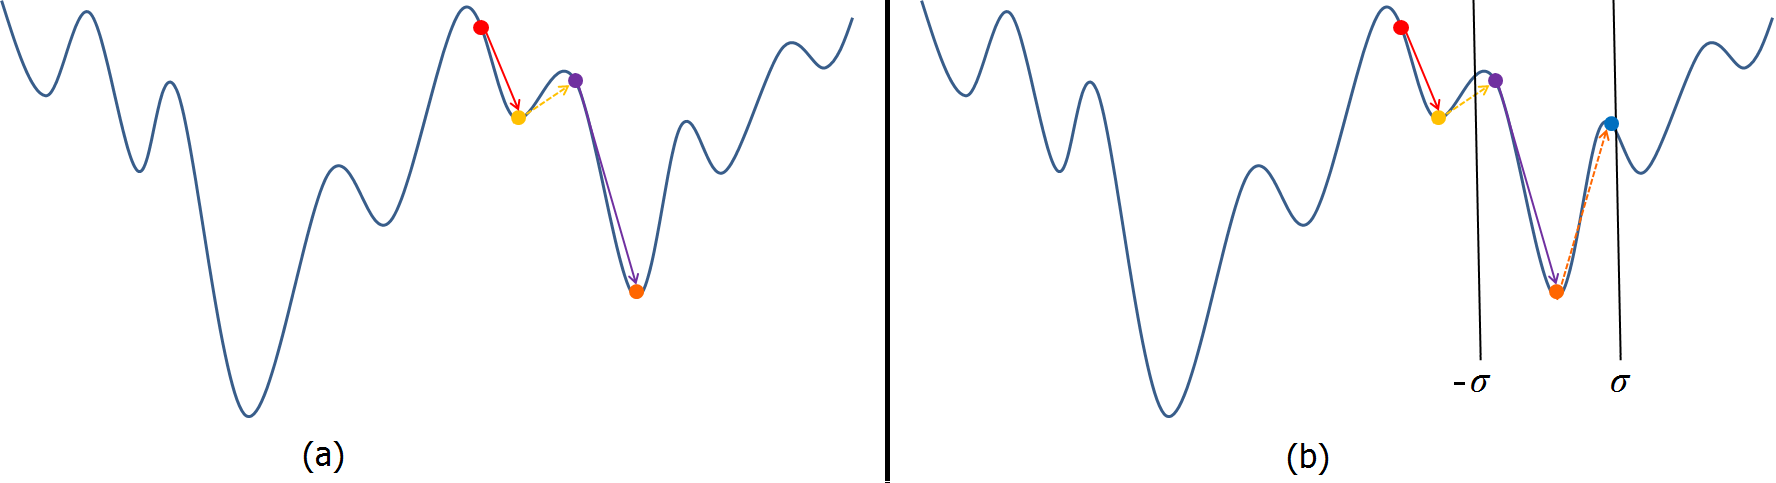
\includegraphics[width=1.0\textwidth]{figures/optimisation/mbh_explained_3.png}
\caption{The third step of \ac{MBH} where (a) the new local minimum $x^{*}$ (orange dot) is compared to the current local minimum $x_{current}$ and is set as $x_{current}$ if it is better. Then (b) the second step repeats from the new $x_{current}$ creating a new perturbed point $x'$ (dark blue dot).}
\label{fig:mbh_explained_3}
\end{figure}

However, it could be possible that at a certain point the minimum does not improve, such as shown in \Cref{fig:mbh_explained_4}. In this case $x_{current}$ is not updated and remains the same, and the loop starts again with the second step, thus perturbing the same minimum point as before. Also, for each consecutive moment that this occurs, $N_{n,i}$ is increased by one. It could be that the minimum value does not improve for a large number of iterations, which means that it is stuck at the best local minimum for that region. \ac{MBH} works with the assumption that basins tend to be close together and thus finds a certain minimum within that set of basins (called a "funnel", which could be the right part of the function curve illustrated in \Cref{fig:mbh_explained_4}). 

\begin{figure}[!ht]
\centering
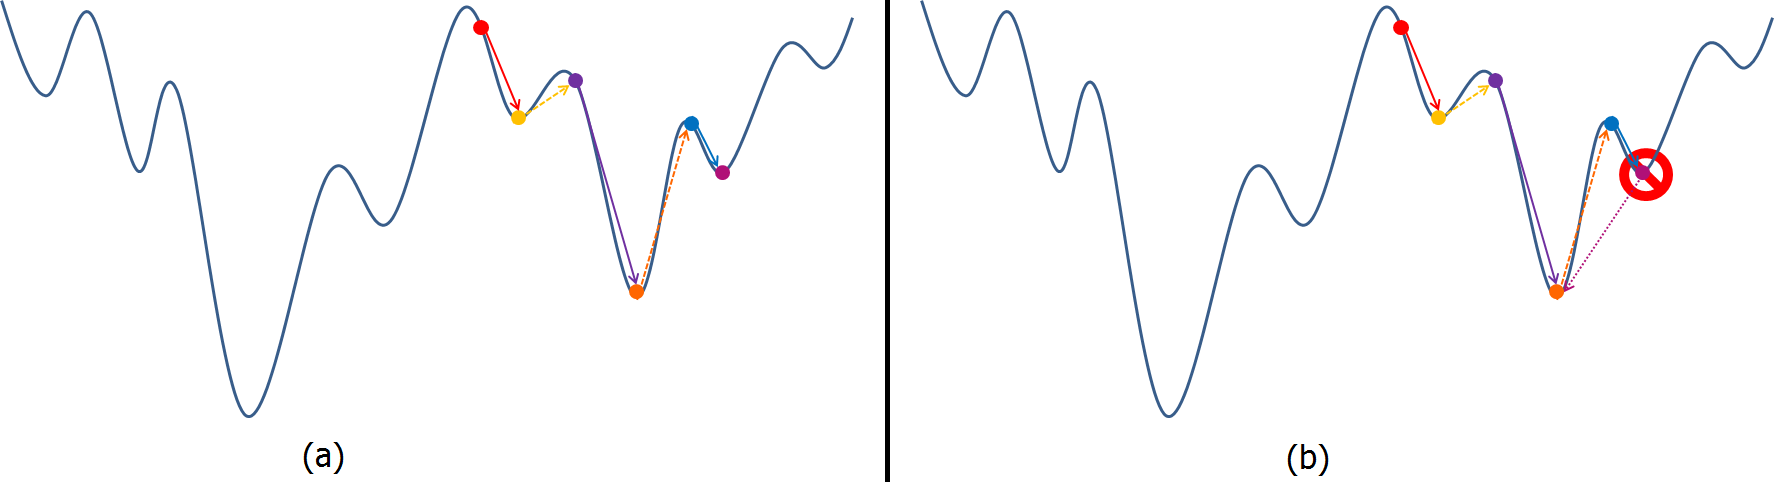
\includegraphics[width=1.0\textwidth]{figures/optimisation/mbh_explained_4.png}
\caption{(a) A new local optimum is found (magenta dot), but (b) it is not better than the current optimum (orange dot), which is why it is disregarded visualized by the dotted arrow.}
\label{fig:mbh_explained_4}
\end{figure}




However, if the minimum point does not improve, it means that it is stuck in such a funnel. The search space however likely contains a number of these funnels, which all have their own best minimum and one of these funnels thus contains the global minimum, which is the minimum that the algorithm attempts to find. So to escape a certain funnel and try to find the next one a maximum on the number of not-improved iterations is set called $Max_{n,i}$. Once this maximum is reached, \ac{MBH} is set to start at the first step again while saving the best found local minimum for that particular funnel. 

%\nomenclature{$Max_{n,i}$}{Maximum number of not improved iterations \nomunit{-}}

This process is repeated (see \Cref{fig:mbh_explained_5}), until either the maximum number of total iterations (steps 1 to 3), or a maximum CPU time is reached. These two criteria are called the cut-off criteria. 

\begin{figure}[!ht]
\centering
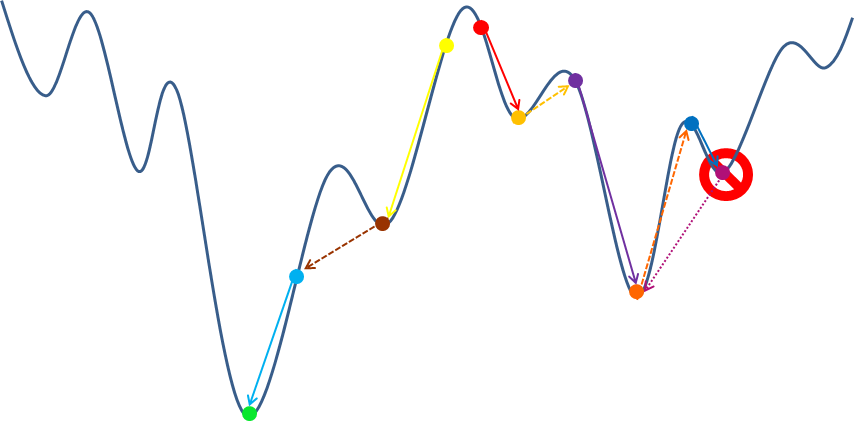
\includegraphics[width=0.5\textwidth]{figures/optimisation/mbh_explained_5.png}
\caption{The process is repeated for another initial guess (yellow dot). In this case, the current funnel contains the global minimum, however the process is still repeated until one of the cut-off criteria has been met.}
\label{fig:mbh_explained_5}
\end{figure}

At the end of the \ac{MBH} run, the best found local minimum is presented and should be the global minimum (unless the global minimum could not be reached before one of the cut-off criteria was met). One of the advantages of this method is that, because \ac{MBH} uses a local optimiser to determine the final values of the variables, the obtained global minimum will be very accurate and convergence to \textit{a} minimum is guaranteed (whether it is the global minimum or not). An example pseudo-code for the described process is provided in \cite{englander2014tuning}. It is thus important to choose a proper local optimiser for \ac{MBH}. The choice of the local optimiser is further discussed in the next section, together with other methods to create variations on the \ac{MBH} method. 



\subsection{Variations of \ac{MBH}}
\label{subsec:varmbhmeth}
There are several ways in which the \ac{MBH} method can be changed.
First the manner in which the values for point $x$ are created can be bound to a certain parameter space for each of the variables. This could result in more feasible points and thus less iterations. Secondly the local optimiser can be chosen by the user themselves depending on the problem that needs to be solved, so different \ac{MBH} methods with different local optimisers can exist. Many reference research that has been focussed on space trajectory problems use the \ac{SNOPT}, such as \cite{yam2011low,englander2012automated,englander2014mars,jamali2009packing} \footnote{The last reference is not a space problem application}. \ac{SNOPT} was introduced in 2002 by Gill et al. \cite{gill2002snopt} as an \ac{SQP} (see \Cref{sec:diffmethloc,sec:techcomp}) method. \ac{SNOPT} requires the first function derivatives and is very effective with highly constrained problems such as trajectory optimisation. More information on the detailed workings of \ac{SNOPT} can be found in \cite{gill2002snopt,gill2006user}. Musegaas \cite{musegaas2012} also mentioned that \ac{SNOPT} should be very useful in future research given the fact that it is a powerful local optimiser. Based on all the reference research and provided that similar problems to the thesis topic have all used or recommended \ac{SNOPT}, this local optimisation tool is chosen to be used in the \ac{MBH} method. Finally, a different distribution from the original uniform probability distribution \cite{jamali2009packing}, used to perturb $x_{current}$, can be used to improve the efficiency and robustness of \ac{MBH}. In \cite{englander2014tuning} two different distributions called Cauchy \footnote{\label{foot:alt_ref_distr} Also used in \cite{englander2012automated}} and bi-polar Pareto $^{\ref{foot:alt_ref_distr}}$ were used to find a better performance of the \ac{MBH} optimiser. In conclusion the paper recommends a bi-polar Pareto distribution, because it improved the performance most compared to the original distribution.







%\nomenclature{}{Description\nomunit{$-$}}